% Options for packages loaded elsewhere
\PassOptionsToPackage{unicode}{hyperref}
\PassOptionsToPackage{hyphens}{url}
%
\documentclass[
  ignorenonframetext,
]{beamer}
\usepackage{pgfpages}
\setbeamertemplate{caption}[numbered]
\setbeamertemplate{caption label separator}{: }
\setbeamercolor{caption name}{fg=normal text.fg}
\beamertemplatenavigationsymbolsempty
% Prevent slide breaks in the middle of a paragraph
\widowpenalties 1 10000
\raggedbottom
\setbeamertemplate{part page}{
  \centering
  \begin{beamercolorbox}[sep=16pt,center]{part title}
    \usebeamerfont{part title}\insertpart\par
  \end{beamercolorbox}
}
\setbeamertemplate{section page}{
  \centering
  \begin{beamercolorbox}[sep=12pt,center]{part title}
    \usebeamerfont{section title}\insertsection\par
  \end{beamercolorbox}
}
\setbeamertemplate{subsection page}{
  \centering
  \begin{beamercolorbox}[sep=8pt,center]{part title}
    \usebeamerfont{subsection title}\insertsubsection\par
  \end{beamercolorbox}
}
\AtBeginPart{
  \frame{\partpage}
}
\AtBeginSection{
  \ifbibliography
  \else
    \frame{\sectionpage}
  \fi
}
\AtBeginSubsection{
  \frame{\subsectionpage}
}
\usepackage{amsmath,amssymb}
\usepackage{lmodern}
\usepackage{iftex}
\ifPDFTeX
  \usepackage[T1]{fontenc}
  \usepackage[utf8]{inputenc}
  \usepackage{textcomp} % provide euro and other symbols
\else % if luatex or xetex
  \usepackage{unicode-math}
  \defaultfontfeatures{Scale=MatchLowercase}
  \defaultfontfeatures[\rmfamily]{Ligatures=TeX,Scale=1}
\fi
\usetheme[]{CambridgeUS}
\usefonttheme{serif}
% Use upquote if available, for straight quotes in verbatim environments
\IfFileExists{upquote.sty}{\usepackage{upquote}}{}
\IfFileExists{microtype.sty}{% use microtype if available
  \usepackage[]{microtype}
  \UseMicrotypeSet[protrusion]{basicmath} % disable protrusion for tt fonts
}{}
\makeatletter
\@ifundefined{KOMAClassName}{% if non-KOMA class
  \IfFileExists{parskip.sty}{%
    \usepackage{parskip}
  }{% else
    \setlength{\parindent}{0pt}
    \setlength{\parskip}{6pt plus 2pt minus 1pt}}
}{% if KOMA class
  \KOMAoptions{parskip=half}}
\makeatother
\usepackage{xcolor}
\newif\ifbibliography
\usepackage{color}
\usepackage{fancyvrb}
\newcommand{\VerbBar}{|}
\newcommand{\VERB}{\Verb[commandchars=\\\{\}]}
\DefineVerbatimEnvironment{Highlighting}{Verbatim}{commandchars=\\\{\}}
% Add ',fontsize=\small' for more characters per line
\usepackage{framed}
\definecolor{shadecolor}{RGB}{48,48,48}
\newenvironment{Shaded}{\begin{snugshade}}{\end{snugshade}}
\newcommand{\AlertTok}[1]{\textcolor[rgb]{1.00,0.81,0.69}{#1}}
\newcommand{\AnnotationTok}[1]{\textcolor[rgb]{0.50,0.62,0.50}{\textbf{#1}}}
\newcommand{\AttributeTok}[1]{\textcolor[rgb]{0.80,0.80,0.80}{#1}}
\newcommand{\BaseNTok}[1]{\textcolor[rgb]{0.86,0.64,0.64}{#1}}
\newcommand{\BuiltInTok}[1]{\textcolor[rgb]{0.80,0.80,0.80}{#1}}
\newcommand{\CharTok}[1]{\textcolor[rgb]{0.86,0.64,0.64}{#1}}
\newcommand{\CommentTok}[1]{\textcolor[rgb]{0.50,0.62,0.50}{#1}}
\newcommand{\CommentVarTok}[1]{\textcolor[rgb]{0.50,0.62,0.50}{\textbf{#1}}}
\newcommand{\ConstantTok}[1]{\textcolor[rgb]{0.86,0.64,0.64}{\textbf{#1}}}
\newcommand{\ControlFlowTok}[1]{\textcolor[rgb]{0.94,0.87,0.69}{#1}}
\newcommand{\DataTypeTok}[1]{\textcolor[rgb]{0.87,0.87,0.75}{#1}}
\newcommand{\DecValTok}[1]{\textcolor[rgb]{0.86,0.86,0.80}{#1}}
\newcommand{\DocumentationTok}[1]{\textcolor[rgb]{0.50,0.62,0.50}{#1}}
\newcommand{\ErrorTok}[1]{\textcolor[rgb]{0.76,0.75,0.62}{#1}}
\newcommand{\ExtensionTok}[1]{\textcolor[rgb]{0.80,0.80,0.80}{#1}}
\newcommand{\FloatTok}[1]{\textcolor[rgb]{0.75,0.75,0.82}{#1}}
\newcommand{\FunctionTok}[1]{\textcolor[rgb]{0.94,0.94,0.56}{#1}}
\newcommand{\ImportTok}[1]{\textcolor[rgb]{0.80,0.80,0.80}{#1}}
\newcommand{\InformationTok}[1]{\textcolor[rgb]{0.50,0.62,0.50}{\textbf{#1}}}
\newcommand{\KeywordTok}[1]{\textcolor[rgb]{0.94,0.87,0.69}{#1}}
\newcommand{\NormalTok}[1]{\textcolor[rgb]{0.80,0.80,0.80}{#1}}
\newcommand{\OperatorTok}[1]{\textcolor[rgb]{0.94,0.94,0.82}{#1}}
\newcommand{\OtherTok}[1]{\textcolor[rgb]{0.94,0.94,0.56}{#1}}
\newcommand{\PreprocessorTok}[1]{\textcolor[rgb]{1.00,0.81,0.69}{\textbf{#1}}}
\newcommand{\RegionMarkerTok}[1]{\textcolor[rgb]{0.80,0.80,0.80}{#1}}
\newcommand{\SpecialCharTok}[1]{\textcolor[rgb]{0.86,0.64,0.64}{#1}}
\newcommand{\SpecialStringTok}[1]{\textcolor[rgb]{0.80,0.58,0.58}{#1}}
\newcommand{\StringTok}[1]{\textcolor[rgb]{0.80,0.58,0.58}{#1}}
\newcommand{\VariableTok}[1]{\textcolor[rgb]{0.80,0.80,0.80}{#1}}
\newcommand{\VerbatimStringTok}[1]{\textcolor[rgb]{0.80,0.58,0.58}{#1}}
\newcommand{\WarningTok}[1]{\textcolor[rgb]{0.50,0.62,0.50}{\textbf{#1}}}
\usepackage{graphicx}
\makeatletter
\def\maxwidth{\ifdim\Gin@nat@width>\linewidth\linewidth\else\Gin@nat@width\fi}
\def\maxheight{\ifdim\Gin@nat@height>\textheight\textheight\else\Gin@nat@height\fi}
\makeatother
% Scale images if necessary, so that they will not overflow the page
% margins by default, and it is still possible to overwrite the defaults
% using explicit options in \includegraphics[width, height, ...]{}
\setkeys{Gin}{width=\maxwidth,height=\maxheight,keepaspectratio}
% Set default figure placement to htbp
\makeatletter
\def\fps@figure{htbp}
\makeatother
\setlength{\emergencystretch}{3em} % prevent overfull lines
\providecommand{\tightlist}{%
  \setlength{\itemsep}{0pt}\setlength{\parskip}{0pt}}
\setcounter{secnumdepth}{-\maxdimen} % remove section numbering
\ifLuaTeX
  \usepackage{selnolig}  % disable illegal ligatures
\fi
\IfFileExists{bookmark.sty}{\usepackage{bookmark}}{\usepackage{hyperref}}
\IfFileExists{xurl.sty}{\usepackage{xurl}}{} % add URL line breaks if available
\urlstyle{same} % disable monospaced font for URLs
\hypersetup{
  pdftitle={Seminário UFSCar, Sorocaba l},
  pdfauthor={Cristian Villegas (clobos@usp.br)},
  hidelinks,
  pdfcreator={LaTeX via pandoc}}

\title{Seminário UFSCar, Sorocaba l}
\author{Cristian Villegas
(\href{mailto:clobos@usp.br}{\nolinkurl{clobos@usp.br}})}
\date{15 de Março de 2023}
\institute{Universidade de São Paulo}

\begin{document}
\frame{\titlepage}

\begin{frame}{What is R?}
\protect\hypertarget{what-is-r}{}
\href{https://www.r-project.org/about.html}{Link for more information}

R is a language and environment for statistical computing and graphics.
It is a \href{https://www.gnu.org/}{GNU project} which is similar to the
S language and environment which was developed at \textbf{Bell
Laboratories} (formerly AT\&T, now Lucent Technologies) by \emph{John
Chambers} and colleagues. R can be considered as a different
implementation of S. There are some important differences, but much code
written for S runs unaltered under R.
\end{frame}

\begin{frame}{What is R?}
\protect\hypertarget{what-is-r-1}{}
R provides a wide variety of statistical (linear and nonlinear
modelling, classical statistical tests, time-series analysis,
classification, clustering, \ldots) and graphical techniques, and is
highly extensible. The S language is often the vehicle of choice for
research in statistical methodology, and R provides an Open Source route
to participation in that activity.
\end{frame}

\begin{frame}{What is R?}
\protect\hypertarget{what-is-r-2}{}
One of R's strengths is the ease with which well-designed
publication-quality plots can be produced, including mathematical
symbols and formulae where needed. Great care has been taken over the
defaults for the minor design choices in graphics, but the user retains
full control.
\end{frame}

\begin{frame}{What is R?}
\protect\hypertarget{what-is-r-3}{}
R is available as Free Software under the terms of the \textbf{Free
Software Foundation's} \href{https://www.r-project.org/COPYING}{GNU
General Public License} in source code form. It compiles and runs on a
wide variety of UNIX platforms and similar systems (including FreeBSD
and Linux), Windows and MacOS.
\end{frame}

\begin{frame}{The R environment}
\protect\hypertarget{the-r-environment}{}
R is an integrated suite of software facilities for data manipulation,
calculation and graphical display. It includes

\begin{itemize}[<+->]
\tightlist
\item
  an effective data handling and storage facility,
\item
  a suite of operators for calculations on arrays, in particular
  matrices,
\item
  a large, coherent, integrated collection of intermediate tools for
  data analysis,
\end{itemize}
\end{frame}

\begin{frame}{The R environment}
\protect\hypertarget{the-r-environment-1}{}
\begin{itemize}[<+->]
\tightlist
\item
  graphical facilities for data analysis and display either on-screen or
  on hardcopy, and
\item
  a well-developed, simple and effective programming language which
  includes conditionals, loops, user-defined recursive functions and
  input and output facilities.
\end{itemize}
\end{frame}

\begin{frame}{The R environment}
\protect\hypertarget{the-r-environment-2}{}
The term ``environment'' is intended to characterize it as a fully
planned and coherent system, rather than an incremental accretion of
very specific and inflexible tools, as is frequently the case with other
data analysis software.
\end{frame}

\begin{frame}{The R environment}
\protect\hypertarget{the-r-environment-3}{}
R, like S, is designed around a true computer language, and it allows
users to add additional functionality by defining new functions. Much of
the system is itself written in the R dialect of S, which makes it easy
for users to follow the algorithmic choices made. For
computationally-intensive tasks, C, C++ and Fortran code can be linked
and called at run time. Advanced users can write C code to manipulate R
objects directly.
\end{frame}

\begin{frame}{The R environment}
\protect\hypertarget{the-r-environment-4}{}
Many users think of R as a statistics system. We prefer to think of it
as an environment within which statistical techniques are implemented. R
can be extended (easily) via packages. There are about eight packages
supplied with the R distribution and many more are available through the
CRAN family of Internet sites covering a very wide range of modern
statistics.
\end{frame}

\begin{frame}{The R environment}
\protect\hypertarget{the-r-environment-5}{}
R has its own LaTeX-like documentation format, which is used to supply
comprehensive documentation, both on-line in a number of formats and in
hardcopy.
\end{frame}

\begin{frame}{Download and Install R}
\protect\hypertarget{download-and-install-r}{}
\href{https://brieger.esalq.usp.br/CRAN/}{Link: The Comprehensive R
Archive Network}

Precompiled binary distributions of the base system and contributed
packages, Windows and Mac users most likely want one of these versions
of R: - Download R for Linux (Debian, Fedora/Redhat, Ubuntu) - Download
R for macOS - Download R for Windows R is part of many Linux
distributions, you should check with your Linux package management
system in addition to the link above.
\end{frame}

\begin{frame}{RStudio}
\protect\hypertarget{rstudio}{}
Used by millions of people weekly, the \textbf{RStudio integrated
development environment (IDE)} is a set of tools built to help you be
more productive with \textbf{R and Python}.
\end{frame}

\begin{frame}{Download RStudio Desktop}
\protect\hypertarget{download-rstudio-desktop}{}
\href{https://posit.co/download/rstudio-desktop/}{link: RStudio Desktop}
\end{frame}

\begin{frame}[fragile]{Install Packages from Repositories or Local
Files}
\protect\hypertarget{install-packages-from-repositories-or-local-files}{}
\begin{Shaded}
\begin{Highlighting}[]
\FunctionTok{install.packages}\NormalTok{(}\StringTok{"tidyverse"}\NormalTok{)}
\end{Highlighting}
\end{Shaded}
\end{frame}

\begin{frame}[fragile]{Loading/Attaching and Listing of Packages}
\protect\hypertarget{loadingattaching-and-listing-of-packages}{}
\begin{Shaded}
\begin{Highlighting}[]
\FunctionTok{library}\NormalTok{(tidyverse)}
\FunctionTok{citation}\NormalTok{(}\StringTok{"tidyverse"}\NormalTok{)}
\end{Highlighting}
\end{Shaded}
\end{frame}

\begin{frame}[fragile]{List Objects (ggplot2 example)}
\protect\hypertarget{list-objects-ggplot2-example}{}
\begin{Shaded}
\begin{Highlighting}[]
\FunctionTok{ls}\NormalTok{(}\StringTok{"package:ggplot2"}\NormalTok{)}
\FunctionTok{citation}\NormalTok{(}\StringTok{"ggplot2"}\NormalTok{)}
\end{Highlighting}
\end{Shaded}
\end{frame}

\begin{frame}[fragile]{Example of dplyr R package}
\protect\hypertarget{example-of-dplyr-r-package}{}
\begin{Shaded}
\begin{Highlighting}[]
\FunctionTok{library}\NormalTok{(dplyr)}
\NormalTok{starwars }\SpecialCharTok{\%\textgreater{}\%} 
  \FunctionTok{select}\NormalTok{(homeworld, height, mass) }
\end{Highlighting}
\end{Shaded}
\end{frame}

\begin{frame}[fragile]{Example of ggplot2 R package}
\protect\hypertarget{example-of-ggplot2-r-package}{}
\begin{Shaded}
\begin{Highlighting}[]
\FunctionTok{library}\NormalTok{(ggplot2)}
\FunctionTok{ggplot}\NormalTok{(mtcars, }\FunctionTok{aes}\NormalTok{(wt, mpg)) }\SpecialCharTok{+} 
  \FunctionTok{geom\_point}\NormalTok{()}
\end{Highlighting}
\end{Shaded}

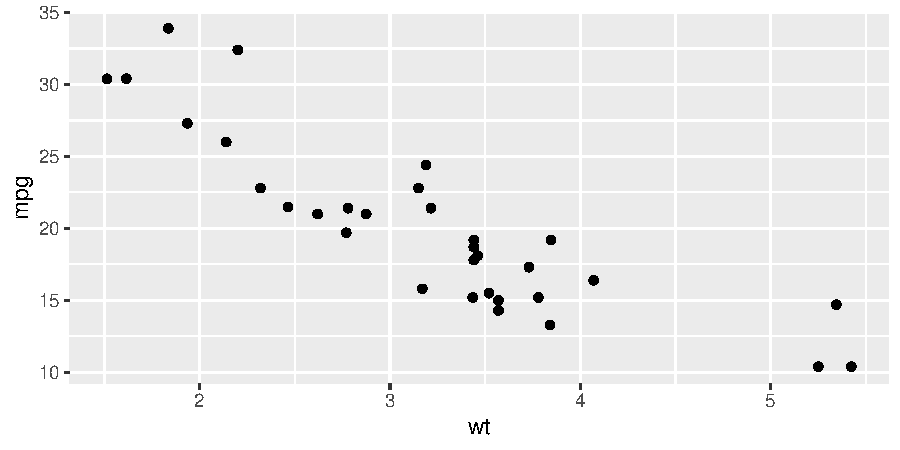
\includegraphics{slides_UFSCar_files/figure-beamer/unnamed-chunk-5-1.pdf}
\end{frame}

\begin{frame}{Rmarkdown from Rstudio}
\protect\hypertarget{rmarkdown-from-rstudio}{}
\begin{itemize}[<+->]
\tightlist
\item
  Documents
\item
  Interactive Documents
\item
  Dashboards
\item
  Presentations
\item
  Books
\item
  Websites
\item
  Templates
\item
  Package Vignettes
\end{itemize}
\end{frame}

\begin{frame}{Rmarkdown from Rstudio: Examples}
\protect\hypertarget{rmarkdown-from-rstudio-examples}{}
\href{https://rmarkdown.rstudio.com/gallery}{Check out the range of
outputs and formats you can create using R Markdown}
\end{frame}

\begin{frame}{Citation R}
\protect\hypertarget{citation-r}{}
To cite R in publications use:

\begin{quote}
R Core Team (2022). R: A language and environment for statistical
computing. R Foundation for Statistical Computing, Vienna, Austria. URL
\url{https://www.R-project.org/}.
\end{quote}
\end{frame}

\begin{frame}{References: Books}
\protect\hypertarget{references-books}{}
\begin{enumerate}[<+->]
[1)]
\item
  \href{https://ggplot2-book.org/}{ggplot2: elegant graphics for data
  analysis, Hadley Wickham}
\item
  \href{https://bookdown.org/rdpeng/rprogdatascience/}{R Programming for
  Data Science, Roger D. Peng}
\item
  \href{https://r4ds.had.co.nz/}{R for Data Science, Hadley Wickham e
  Garrett Grolemund.}
\item
  \href{https://r-graphics.org/}{R Graphics Cookbook, Winston Chang}
\end{enumerate}
\end{frame}

\begin{frame}{References (links do dplyr, ggplot2 e magrittr)}
\protect\hypertarget{references-links-do-dplyr-ggplot2-e-magrittr}{}
\begin{enumerate}[<+->]
[1)]
\item
  \href{https://dplyr.tidyverse.org/}{Link: dplyr do tidyverse}
\item
  \href{https://ggplot2.tidyverse.org/}{Link: ggplot2 do tidyverse}
\item
  \href{https://magrittr.tidyverse.org/}{Link: magrittr do tidyverse?}
\end{enumerate}
\end{frame}

\begin{frame}{Reference: cheat sheet}
\protect\hypertarget{reference-cheat-sheet}{}
\begin{enumerate}[<+->]
[1)]
\item
  \href{https://github.com/rstudio/cheatsheets/blob/main/data-visualization.pdf}{Link
  Data visualization with ggplot2}
\item
  \href{https://github.com/rstudio/cheatsheets/blob/main/data-transformation.pdf}{Link
  Data transformation with dplyr}
\item
  \href{https://github.com/rstudio/cheatsheets/blob/main/rmarkdown.pdf}{Link
  Rmarkdown}
\item
  \href{https://github.com/rstudio/cheatsheets/blob/main/rstudio-ide.pdf}{Link
  Rstudio IDE}
\end{enumerate}
\end{frame}

\end{document}
